\documentclass[11pt]{article}            % Report class in 11 points
\parindent0pt  \parskip10pt             % make block paragraphs
\usepackage{graphicx}
\usepackage{listings}
\usepackage[document]{ragged2e}
\usepackage{float}
\newcommand\tab[1][1cm]{\hspace*{#1}}
\graphicspath{ {images/} }
\usepackage{graphicx} %  graphics header file
\begin{document}
\begin{titlepage}
    \centering
  \vfill
    
\includegraphics[width=8cm]{uni_logo.png} \\ 
	\vskip2cm
    {\bfseries\Large
	Data Structures  \& Algorithms \\ (CS09203)\\
	
	\vskip2cm
	Lab Report 
	 
	\vskip2cm
	}    

\begin{center}
\begin{tabular}{ l l  } 

Name: & Muhammad Umer \\ 
Registration \#: & CSU-F16-104 \\ 
Lab Report \#: & 04 \\ 
 Dated:& 23-04-2018\\ 
Submitted To:& Mr. Usman Ahmed\\ 

 %\hline
\end{tabular}
\end{center}
    \vfill
    The University of Lahore, Islamabad Campus\\
Department of Computer Science \& Information Technology
\end{titlepage}


    
    {\bfseries\Large
\centering
	Experiment \# 1 \\

Link List-Basic Insertion and Traversal\\
	
	}    
 \vskip1cm
 \textbf {Objective}\\  To understand and implement the Link List with basic Insertion and Traversal.
 
 \textbf {Software Tool} \\
1. Sublime Text Editor\\
2. Dev C++\\
3. Window 7 (32 Bit)\\

\section{Theory }              
\justify One disadvantage of using arrays to store data is that arrays are static structures and therefore cannot be easily extended or reduced to fit the data set. Arrays are also expensive to maintain new insertions and deletions. In this chapter we consider another data structure called Linked Lists that addresses some of the limitations of arrays.\\~\\
A linked list is a linear data structure where each element is a separate object.\\~\\
\begin{figure}[H]
\centering
  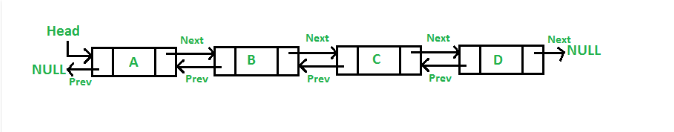
\includegraphics[width=12cm,height=6cm,keepaspectratio]{5.png}    
\end{figure}
Each element (we will call it a node) of a list is comprising of two items - the data and a reference to the next node. The last node has a reference to null. The entry point into a linked list is called the head of the list. It should be noted that head is not a separate node, but the reference to the first node. If the list is empty then the head is a null reference.\\~\\
A linked list is a dynamic data structure. The number of nodes in a list is not fixed and can grow and shrink on demand. Any application which has to deal with an unknown number of objects will need to use a linked list.\\~\\
One disadvantage of a linked list against an array is that it does not allow direct access to the individual elements. If you want to access a particular item then you have to start at the head and follow the references until you get to that item.
\section{Task}  
\subsection{Procedure: Task 1 Insertion}

In this Linked List user can insert integer type of the data and the data will always be inserted in the start of the list.  

\begin{lstlisting}[language=C++]

 
void insert(int item){
	node *NewNode = (node*) malloc(sizeof(node));
	NewNode -> data = item;
	NewNode -> next = head;
	head = NewNode;
}
\end{lstlisting}   

\begin{figure*}
\centering
  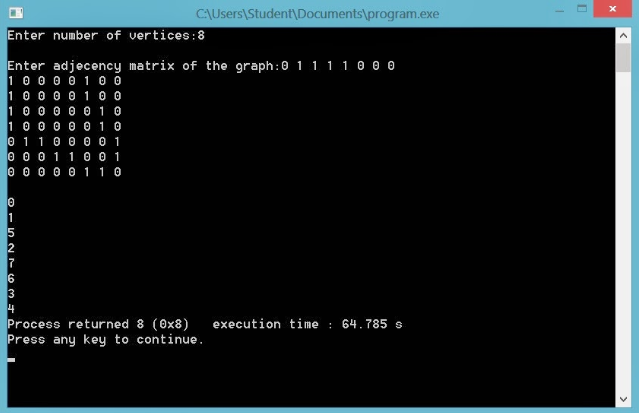
\includegraphics[width=12cm,height=6cm,keepaspectratio]{1.png}
\caption{Time Independent Feature Set}
\label{Figure:3}    
\end{figure*}

\subsection{Procedure: Task 2 Display}     

\begin{lstlisting}[language=C++]
void display(){
	if(head == NULL){
		cout<<"\n\nError: Empty List!";
		cout<<"\n\nPress any key to continue...";
		getch();
		return;
	}
	node *NewNode = (node*) malloc(sizeof(node));
	NewNode = head;
	cout<<"\n\nData in the List:\n\n";
	while(NewNode != NULL){
		cout<<NewNode -> data<<" ";
		NewNode = NewNode -> next;
	}
}
\end{lstlisting}

\section{Program}
\begin{lstlisting}[language=C++]

#include<iostream>
#include<stdlib.h>
#include<conio.h>
using namespace std;

struct node{
	int data;
	node* next;
};

node* head = NULL;

void insert(int item){
	node *NewNode = (node*) malloc(sizeof(node));
	NewNode -> data = item;
	NewNode -> next = head;
	head = NewNode;
	cout<<"\n\nData Inserted Successfully!";
	cout<<"\n\nPress any key to continue...";
	getch();
}

void display(){
	if(head == NULL){
		cout<<"\n\nError: Empty List!";
		cout<<"\n\nPress any key to continue...";
		getch();
		return;
	}
	node *NewNode = (node*) malloc(sizeof(node));
	NewNode = head;
	cout<<"\n\nData in the List:\n\n";
	while(NewNode != NULL){
		cout<<NewNode -> data<<" ";
		NewNode = NewNode -> next;
	}
	cout<<"\n\nPress any key to continue...";
	getch();
}

int main(){
	int choice, item;
	up:
	system("cls");
	cout<<"\n\n\tCHOOSE FROM THE FOLLOWING:";
	cout<<"\n\n\t1. Insert Data in the List";
	cout<<"\n\t2. Display Data of the List";
	cout<<"\n\t3. Exit\n\n\t";
	cin>>choice;
	if(choice == 1){
		cout<<"\n\nEnter a value: ";
		cin>>item;
		insert(item);
		goto up;
	}
	else if(choice == 2){
		display();
		goto up;
	}
	else if(choice == 3){
		exit(0);
	}
	else{
		cout<<"\n\nWRONG CHOICE!";
		cout<<"\n\nPress any key to choose again...";
		getch();
		goto up;
	}
	return 0;
	
}
\end{lstlisting}

\section{Output}
\begin{figure}[H]
\centering
  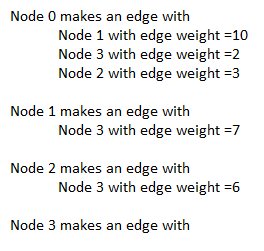
\includegraphics[width=12cm,height=6cm,keepaspectratio]{2.png}
\caption{Main Menu and Insertion}
\label{Figure:2}    
\end{figure}

\begin{figure}[H]
\centering
  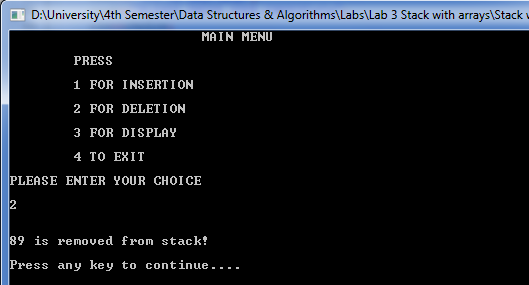
\includegraphics[width=12cm,height=6cm,keepaspectratio]{3.png}
\caption{Displaying List}
\label{Figure:3}    
\end{figure}

\begin{figure}[H]
\centering
  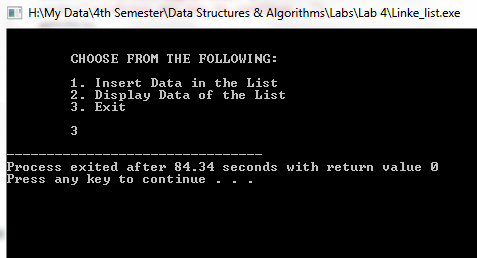
\includegraphics[width=12cm,height=6cm,keepaspectratio]{4.png}
\caption{Exit}
\label{Figure:4}
\end{figure}

 \textbf {Source Code} \\


\section{Conclusion}
A linked list is a linear data structure where each element is a separate object. Each element is called as a node, that contains two item - the data and a reference to the next node. The last node has a reference to null. The entry point into a linked list is called the head of the list. A linked list is a dynamic data structure. The number of nodes in a list is not fixed and can grow and shrink on demand.\\~\\

\tab[6cm] \noindent\rule{6cm}{0.4pt}\\
\tab[6cm] (Concerned Teacher/Lab Engineer)


 
\end{document}                          % The required last line
